%----------------------------------------------------------------------------------------
%	Packages
%----------------------------------------------------------------------------------------

\documentclass[11pt]{diazessay} % Font size (can be 10pt, 11pt or 12pt)

%----------------------------------------------------------------------------------------
%	Title
%----------------------------------------------------------------------------------------

\title{\textbf{Dynamics Of Celestial Bodies In Space}} % Title and subtitle
\author{\textbf{Taylor Larrechea} \\ \textit{Colorado Mesa University}} % Author and institution
\date{March 12, 2026} %Date

%----------------------------------------------------------------------------------------
%	Begin Document
%----------------------------------------------------------------------------------------

\begin{document}
\maketitle % Print the title section

%----------------------------------------------------------------------------------------
%	Abstract
%----------------------------------------------------------------------------------------

\begin{abstract}
This work presents a computational study of the dynamics of celestial bodies governed by Newtonian gravitation. The equations of motion are derived and numerically integrated to analyze two-body, 
three-body, and general N-body systems. The original Python implementation was refactored into C++ to improve performance and structural clarity. In addition, a neural network model was developed to 
approximate dynamical behavior in projectile motion systems. A generalized N-body solver was implemented to extend the framework beyond classical three-body configurations, enabling scalable simulation 
of multi-body gravitational interactions.
\end{abstract}

%----------------------------------------------------------------------------------------
%	Document
%----------------------------------------------------------------------------------------
\begin{center}
\begin{figure}[htpb]
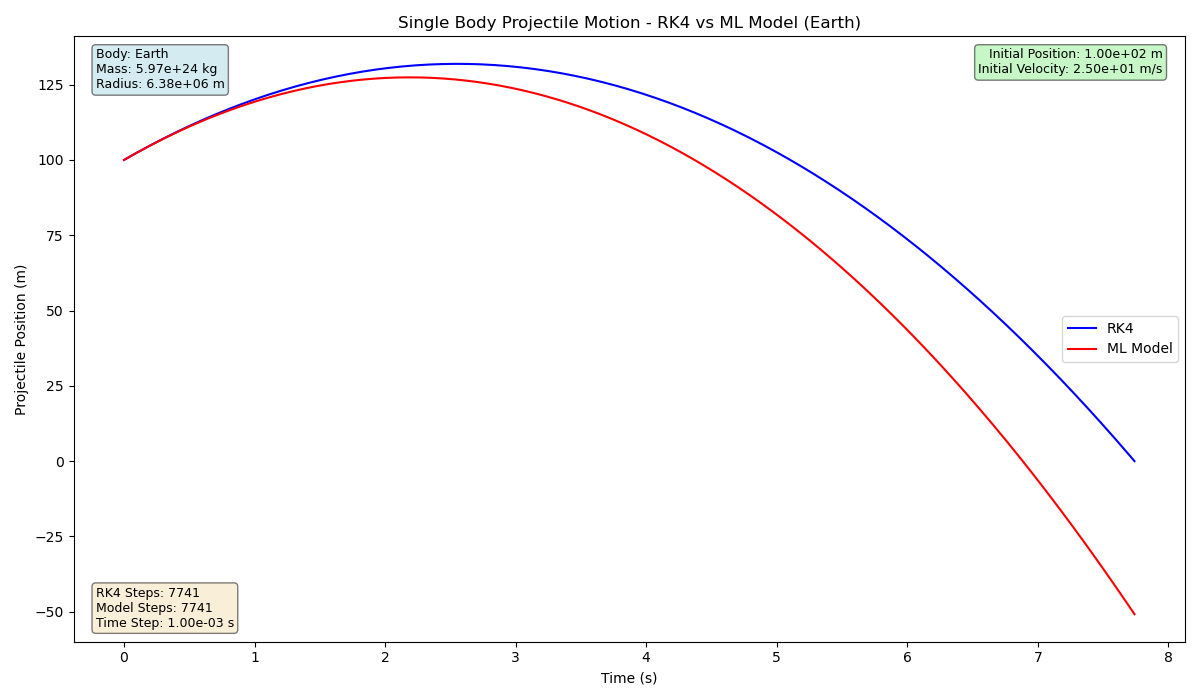
\includegraphics[width=1.00\linewidth]{Figures/MLPrediction.png}
\end{figure}
\end{center}

\href{https://github.com/QuantumCompiler/Dynamics-Of-Celestial-Bodies}{\textbf{Quantum Compiler - Dynamics Of Celestial Bodies Repository}}

\end{document}

%----------------------------------------------------------------------------------------
%	Comment Headers
%----------------------------------------------------------------------------------------

%----------------------------------------------------------------------------------------
%	
%----------------------------------------------------------------------------------------